%\documentclass[12pt,letterpaper]{amsart}
%\setlength{\oddsidemargin}{.0in}
%\setlength{\evensidemargin}{.0in}
%\setlength{\textwidth}{6.5in}
%\setlength{\topmargin}{-.3in}
%\setlength{\headsep}{.20in}
%\setlength{\textheight}{9.in}
%\usepackage[leqno]{amsmath}
%\usepackage{amsfonts}
%\usepackage{amssymb}
%\usepackage{amsthm}
%\usepackage{amssymb}
%\usepackage[all]{xy}
%\usepackage{graphicx}



%Here are some user-defined notations
\newcommand{\RR}{\mathbf R}
\newcommand{\CC}{\mathbf C}
\newcommand{\ZZ}{\mathbf Z}
\newcommand{\ZZn}[1]{\ZZ/{#1}\ZZ}
\newcommand{\QQ}{\mathbf Q}
\newcommand{\rr}{\mathbb R}
\newcommand{\cc}{\mathbb C}
\newcommand{\zz}{\mathbb Z}
\newcommand{\zzn}[1]{\zz/{#1}\zz}
\newcommand{\qq}{\mathbb Q}
\newcommand{\calM}{\mathcal M}
\newcommand{\latex}{\LaTeX}
\newcommand{\tex}{\TeX}
\newcommand{\sm}{\setminus} 

%\newtheorem{example}[theorem]{Example}
%\newtheorem{remark}[theorem]{Remark}
%improving spacing in tables (space above and below characters in a row)
\newcommand{\tfix}{\rule{0pt}{2.6ex}}
\newcommand{\bfix}{\rule[-1.2ex]{0pt}{0pt}}



%Here are commands with variable inputs 
\newcommand{\intf}[1]{\int_a^b{#1}\,dx}
\newcommand{\intfb}[3]{\int_{#1}^{#2}{#3}\,dx}
\newcommand{\marginalfootnote}[1]{%
        \footnote{#1}
        \marginpar[\hfill{\sf\thefootnote}]{{\sf\thefootnote}}}
\newcommand{\edit}[1]{\marginalfootnote{#1}}


%Here are some user-defined operators
\newcommand{\Tr}{\operatorname {Tr}}
\newcommand{\GL}{\operatorname {GL}}
\newcommand{\SL}{\operatorname {SL}}
\newcommand{\Prob}{\operatorname {Prob}}
\newcommand{\re}{\operatorname {Re}}
\newcommand{\im}{\operatorname {Im}}


%These commands deal with theorem-like environments (i.e., italic)
%\theoremstyle{plain}
%\newtheorem{theorem}{Theorem}[section]
%\newtheorem{corollary}[theorem]{Corollary}
%\newtheorem{lemma}[theorem]{Lemma}
%\newtheorem{conjecture}[theorem]{Conjecture}

%These deal with definition-like environments (i.e., non-italic)
%\theoremstyle{definition}
%\newtheorem{definition}[theorem]{Definition}


%This numbers equations by section
\numberwithin{equation}{section}

\section{Stochastics}
\begin{frame}
  \frametitle{Outline}
  \tableofcontents[ currentsection ]
\end{frame}

\subsection{Fundamental Concepts}
%\begin{document}
\begin{frame}{Markov Process}
(\textbf{Markov Process}) is a stochastic process with the following properties: 
\begin{enumerate}
\item The outcome at any stage depends only on the outcome of the previous stage.
\item The probabilities are constant over time.   
\end{enumerate}
\end{frame}


\begin{frame}{Brownian Motion}
\begin{definition}(\textbf{Brownian Motion}) is a stochastic process that models random continuous motion. The stochastic process $B=\{B(t), t\geq 0\}$ is standard Brownian Motion if the following holds:
\begin{enumerate}
\item $B$ has independent increments.
\item For $0 \leq s < t,$ $$B(t)-B(s) \sim N(0,t-s).$$
\item The paths of $B$ are continuous with probability $1$.
\item $B(0)=0$ 
\end{enumerate}
\end{definition}
\end{frame}

\begin{frame}
  %\frametitle{Without Noise}
  %\movie[height=6.33cm,width=8.55cm,loop,poster]{Random Walk}{randomWalk.mp4}
\vfill

%\begin{center}
	%\includemedia[
	%	label=vidA,
	%	addresource=randomWalk.mp4,
	%	activate=pageopen,
	%	width=10cm, height=8cm,
	%	flashvars={
	%		source=randomWalk.mp4
	%		&loop=true}
	%	]{}{VPlayer.swf}
%\end{center}

%\vfill
  %\hyperlinkmovie[once]{randomWalk.mp4}{Random Walk} 
  %\cite{doi:10.1137/S0036144500378302}
\end{frame}

\begin{frame}
   \frametitle{Monte Carlo Simulation - Brownian Motion}
	Recorded final step of 5000 Brownian Motions over [0,1]\\
	We expect the distribution to be $~N(0,1)$. \\
	\begin{center}
		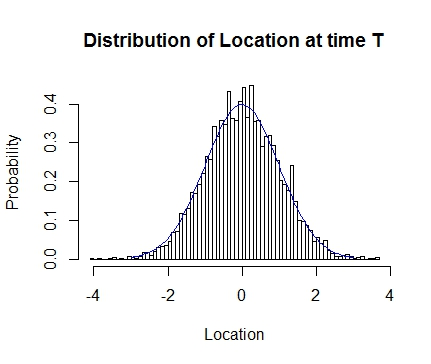
\includegraphics[width=5cm]{img/bpath1montecarlohist}\\
	\end{center}
	\begin{center}
	$\bar{x}=0.019311,\hspace{1em} s^{2}=0.9933$,\hspace{1em} $t-test \hspace{.5em} p-value=0.16924$ 
	\end{center} 
	\centerline{CI:\hspace{1em}  $\mu\hspace{.5em}\epsilon \hspace{.5em}(-0.00822 , 0.046844)$}
\end{frame}

\begin{frame}{Monte Carlo Simulation - Approximations}
Carrie inserts her stuff here. 
\end{frame}


\begin{frame}{Scaling a Brownian Motion}
\vfill

If $x(t)$ is a Brownian Motion then 
$\displaystyle \frac{x(\lambda t)}{\sqrt{\lambda}}$ 
is a Brownian motion.
	
\vfill
\begin{eqnarray*}
  \lefteqn{
	P \left(a \leq \frac{x(\lambda t)}{\sqrt{\lambda}}-\frac{x(\lambda s)}{\sqrt{\lambda}} \leq b \right)
	} & & \\
    & = & P \left(a \sqrt{\lambda} \leq x(\lambda t) - x (\lambda s) \leq b \sqrt{\lambda} \right), \\
	& = & \displaystyle \frac{1}{\sqrt{2 \pi (\lambda t -\lambda s)}} 
                    \int_{a \sqrt{\lambda}}^{b \sqrt{\lambda}} e^{\frac{-x^2}{2}(\lambda t- \lambda s)} dx, \\
    & = & \frac{1}{\sqrt{2 \pi (t-s)}} \int_{a}^{b} e^{\frac{-u^2}{t-s}}du.
 \end{eqnarray*}
\end{frame}

\subsection{Integration}
%\begin{frame}{Riemann-Stieltjes}
%(\textbf{Riemann-Stieltjes Integral}): 
%$$\displaystyle \int_{a}^{b} f(g)dg= \underset{n \to \infty}{\lim} \sum_{i=1}^{N} f(g(t_i)) \cdot (g(t_{i+1}))- g(t_i))$$\\

%The main motivation for the Riemann-Stieltjes Integral comes from the concept of Cumulative Distribution Function (CDF) of a random variable. 
%\end{frame}

\begin{frame}{Wiener Process}
A standard Wiener process (also called Brownian Motion) is a stochastic process $\{W_t\}_{t \geq 0},$ which has properties mutually consistent with those of Brownian motion.

\vfill

\textbf{Wiener Integral} For a pair $(W_t,f(t))$ of a Wiener Process $W_t,$ a random process $f(t),$ we define the It\^o integral 
	$$I(f)=\int_0^{a} f(t)dW_t$$
\end{frame}

\begin{frame}
   \frametitle{Monte Carlo Simulation - It\^o Integral}
	Recorded approximations of 5000 It\^o Integrals for $\int^{1.5}_{0} W dW$\\
	WHAT DO WE EXPECT???? I DON'T KNOW. \\
	\begin{center}
		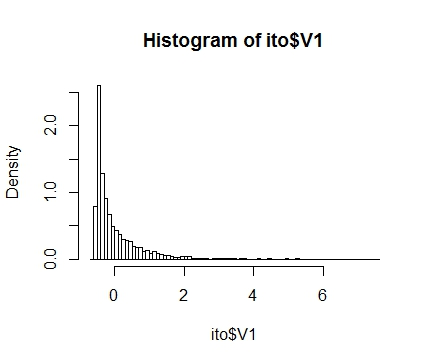
\includegraphics[width=5cm]{img/ito}\\
	\end{center}
	\begin{center}
	$\bar{x}=0.000555,\hspace{1em} s^{2}=0.4925248$%,\hspace{1em} $t-test \hspace{.5em} p-value=0.16924$ 

%GUYS...... NOW THAT YOU'RE HERE---- LOOK AT ito_integral_stats.R. We expect mean 0 and variance .5??????????
% AND I'M NOT SURE IF THE CONFIDENCE INTERVAL WORKS RIGHT FOR THIS EITHER!!
	\end{center} 
	%\centerline{CI:\hspace{1em}  $\mu\hspace{.5em}\epsilon \hspace{.5em}(-0.00822 , 0.046844)$}
\end{frame}


%\textbf{Multivariate Taylor Expansion:} $$F(t)-F(s)=F^{\prime}(s)(t-s)+\frac{1}{2}F^{''} (s)(t-s)^2 + \frac{1}{3!}F^{'''}(t-s)^3+ \text{H.O.T}$$

\subsection{It\^o's Formula}

\begin{frame}
\frametitle{It\^o's Formula}
It\^o's Formula is used in It\^o Calculus to find the differential of a time-dependent function of a stochastic process.
\vfill

		 \begin{block}{Differential Form}
      \begin{align*}
				\displaystyle dx_t =\left(\frac{\partial x}{\partial t} + \frac{1}{2} \left(\frac{\partial ^2 x}{\partial B ^2}\right)\right) \cdot  dt + \frac{\partial x}{\partial B} \cdot dB 
			\end{align*}
    \end{block}
		
\vfill

		\begin{block}{Integral Form}
      \begin{align*}
				\displaystyle F(t, B(t))-F(a,B(a))=
 \int_{a}^{t} \frac{\partial F}{\partial s} + \frac{1}{2} \frac{\partial^2 F}{\partial B^2}ds+
 \int_a^t \frac{\partial F}{\partial B} dB
			\end{align*}
    \end{block}

\vfill
\end{frame}

\begin{frame}{It\^o's Formula} 

Let $F=tB^2$ 
\begin{align*}
\displaystyle
\frac{\partial F}{\partial t}&= B^2\\
\frac{\partial F}{\partial B}&=2t \cdot B\\ 
\frac{\partial^2 F}{\partial B^2}&=2t
\end{align*}
\begin{align*}
tB^2(t)-aB^2(a) &=\int_{a}^{t}B^2 ~ ds+ \int_{a}^{t}2sB ~ dB+\int_a^t \frac{1}{2}2s ~ ds\\
 &\text{OR}\\
tB^2(t)-aB^2(a) &= \int_a^t B^2 ~ ds+ \int_a^t 2sB ~ dB+ \frac{1}{2} t^2- \frac{1}{2}a^2
\end{align*}
\end{frame}

%\section{Nondimensionalization}
%\begin{frame}
 % \frametitle{Outline}
  %\tableofcontents[ currentsection ]
%\end{frame}

%\begin{frame}{Nondimensionalization}
%\textbf{Nondimensionalization}: method to reduce parameters. 

%\begin{enumerate}
%\item
%List all the variables and parameters along with their dimensions.
%\item
%For each variable, say $x$, form a product (or quotient) $p$ of parameters that has the same dimensions as $x$, and define a new variable $y=\frac{x}{p}.$ $y$ is a "dimensionless" variable. It's numberical  value is the same no matter what system of units is used.
%\item Rewrite the differential equation in terms of the new variables.
%\item 
%In the new differential equation, group the parameters into nondimensional combinations, and define a new set of nondimensional parameters expressed as the nondimensional combinations of the original parameters. 
%\end{enumerate}
%\end{frame}


%\end{document}

